% ============================================================
% Lecture 7 -- Play with more data sets in R
% ============================================================
\section{Playing with More Data Sets}\label{sec:L07}

\lectureheader{7}{V8SQrXbSA44}{Week-2 slides \texttt{Feb2.pdf} (smallmouth bass and snowfall examples), with annotations; Week-2 data sets \texttt{wblake.txt}, \texttt{snow.txt}}

\begin{guiding*}
By the end of this lecture you should be able to:
\begin{itemize}
  \item explore a data set with a discrete explanatory variable (age) and compare the mean response at each level with a fitted line;
  \item explain why a regression of $y$ on $x$ cannot simply be inverted to predict $x$ from $y$;
  \item recognise from a scatter plot and a fitted line when two variables are essentially unrelated.
\end{itemize}
\end{guiding*}

\subsection{Recap}
We can fit a least-squares line (\cref{sec:L05}) and check it with a residual plot
(\cref{sec:L06}). The instructor now applies the same steps to further data sets from
Weisberg's book. The point is to see how scatter plots guide the choice of a model.

\subsection{Length at age for smallmouth bass}
\begin{example}[West Bearskin Lake bass]\label{ex:L07-bass}
The data (\texttt{wblake.txt}; \texttt{wblake} in \texttt{alr4}) record the \texttt{Length}
(mm) and \texttt{Age} (years) of $n=439$ smallmouth bass caught in West Bearskin Lake, Minnesota,
USA, in 1991. Age is determined from annular rings on the fish's scales, like the rings of a
tree. Ages run from $1$ to $8$, with counts
\begin{center}
\begin{tabular}{lcccccccc}\hline
Age & 1 & 2 & 3 & 4 & 5 & 6 & 7 & 8\\
number of fish & 38 & 72 & 94 & 15 & 68 & 87 & 61 & 4\\\hline
\end{tabular}
\end{center}
\end{example}

Because Age is discrete, the scatter plot consists of eight vertical strips. Within each strip
there is a spread of lengths. Fish of the same age differ in length. We can summarise each strip
by its mean length and compare the eight means with the least-squares line
\[
\widehat{\text{Length}} = 65.53 + 30.32\,\text{Age}.
\]
The means lie close to the line for young fish but bend below it for the oldest: growth slows
with age. The instructor's annotation makes a second point. The graph shows how length
depends on age, but \emph{we cannot use the line to predict age from length}. Each strip is wide,
and the strips overlap heavily. A fish of length $200$\,mm could plausibly be $3$, $4$ or $5$
years old. Moreover, inverting the line $y=a_1+a_2x$ is not the same as regressing $x$ on $y$.

\begin{proposition}[Supplementary: regression is not symmetric]\label{prop:L07-asym}
Let $\hat a_2^{(y|x)}=S_{xy}/S_{xx}$ be the least-squares slope of $y$ on $x$ and
$\hat b_2^{(x|y)}=S_{xy}/S_{yy}$ the slope of $x$ on $y$. Then
\[
\hat a_2^{(y|x)}\cdot \hat b_2^{(x|y)}=r^2,\qquad r=\frac{S_{xy}}{\sqrt{S_{xx}S_{yy}}} .
\]
The line of $y$ on $x$, rewritten as a line for $x$ in terms of $y$, has slope $1/\hat a_2^{(y|x)}$.
This equals $\hat b_2^{(x|y)}$ only when $r^2=1$, i.e.\ when all points lie exactly on a line.
\end{proposition}
\begin{proof}
Both formulas come from \cref{thm:L05-slr}, with the roles of $x$ and $y$ swapped for the second.
Multiplying, $\hat a_2\hat b_2 = S_{xy}^2/(S_{xx}S_{yy})=r^2$. The equality
$1/\hat a_2=\hat b_2$ is equivalent to $\hat a_2\hat b_2=1$, i.e.\ to $r^2=1$. By the
Cauchy--Schwarz inequality $r^2\le 1$, with equality if and only if the vectors
$(y_i-\bar y)$ and $(x_i-\bar x)$ are proportional.
\end{proof}

\subsection{Predicting the weather: snowfall}
\begin{example}[Fort Collins snowfall]\label{ex:L07-snow}
Can the snowfall of early winter predict the snowfall of late winter? The data (\texttt{snow.txt};
\texttt{ftcollinssnow} in \texttt{alr4}) give, for $93$ years starting in 1900 at Fort Collins,
Colorado, the snowfall (inches) from September to December (\texttt{Early}) and from January to
June (\texttt{Late}).
\end{example}
The scatter plot of Late against Early is a shapeless cloud. The least-squares line is
\[
\widehat{\text{Late}} = 28.64 + 0.2035\,\text{Early},
\]
with $R^2=0.0258$ and sample correlation $r=0.161$. The slope is small and, as we will be able to
test in \cref{sec:L16}, not significantly different from $0$ (p-value $0.124$). The fitted line
is hardly distinguishable from the horizontal line at the mean of Late. The instructor's
conclusion, written on the slide: early and late snowfall are \emph{not related}.
A good-looking line can always be computed. Whether it means anything is a separate question.

\begin{figure}[ht]
\centering
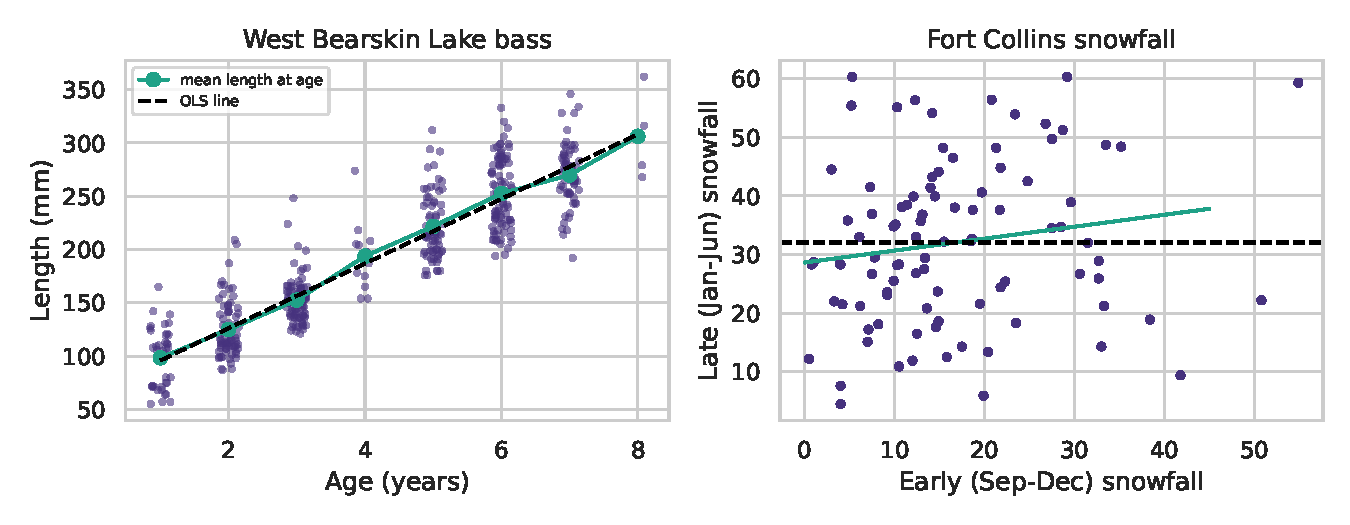
\includegraphics[width=0.95\textwidth]{figures/L07_bass_snow.pdf}
\caption{Left: bass length against age, with mean length at each age and the least-squares line.
Right: late against early snowfall; the fitted line (solid) is close to the mean of Late (dashed).}
\label{fig:L07-bass-snow}
\end{figure}

\subsection{Computation}
The Week-2 R code reads each \texttt{.txt} file, plots it and calls \texttt{lm}. In Python:
\codeline{w = pd.read\_csv(DATA / "wblake.csv"); w.groupby("Age").Length.mean(); smf.ols("Length \textasciitilde\ Age", w).fit()}
\codeline{sn = pd.read\_csv(DATA / "ftcollinssnow.csv"); smf.ols("Late \textasciitilde\ Early", sn).fit().summary()}
See \nb{week02/L07\_more\_datasets.ipynb}.

\subsection{Summary}
\begin{itemize}
  \item Bass: $\widehat{\text{Length}}=65.53+30.32\,\text{Age}$. Mean length grows with age but levels off. Age cannot be predicted reliably from length.
  \item The regressions of $y$ on $x$ and of $x$ on $y$ differ unless $r^2=1$. Their slopes multiply to $r^2$.
  \item Snowfall: slope $0.2035$, $R^2=0.026$. Early and late snowfall are essentially unrelated.
\end{itemize}

\subsection{Exercises}
\begin{problem}\label{prob:L07-1}
Compute the least-squares line of Age on Length for the bass data and compare its slope with $1/30.32$.
\end{problem}
\begin{problem}\label{prob:L07-2}
Show that $\hat a_2=r\, s_y/s_x$, where $s_x,s_y$ are the sample standard deviations.
\end{problem}
\begin{problem}\label{prob:L07-3}
For the snowfall data, compute $\sum_i(\text{Late}_i-\overline{\text{Late}})^2$ and the minimum of $f$ from \cref{thm:L05-slr}. What fraction of the total is removed by the line?
\end{problem}
\begin{problem}\label{prob:L07-4}
Fit a model in which each age has its own mean length (use \texttt{C(Age)} in the formula). Compare its residual sum of squares with that of the straight line. Which is smaller, and why must it be?
\end{problem}

\subsection{Further reading}
Weisberg, \emph{ALR}, Chapter~1 (bass and snowfall examples). Christensen, Chapter~6
(Regression) and Chapter~4 (one-way ANOVA, the ``one mean per age'' model).
